\documentclass[aps,prx,reprint,raggedbottom,superscriptaddress,longbibliography,floatfix]{revtex4-2}
\usepackage[T1]{fontenc}
\usepackage[utf8]{inputenc}
\usepackage{lmodern,graphicx,booktabs,amsmath,amssymb,microtype,xcolor}
\usepackage{tikz}
\usetikzlibrary{arrows.meta}
\usepackage[colorlinks=true,urlcolor=blue!55!black,linkcolor=blue!55!black,citecolor=blue!55!black]{hyperref}
\setcounter{dbltopnumber}{5}
\setcounter{topnumber}{5}
\setcounter{totalnumber}{8}
\renewcommand{\dbltopfraction}{0.95}
\renewcommand{\topfraction}{0.95}
\renewcommand{\textfraction}{0.05}
\setlength{\tabcolsep}{4pt}
\renewcommand{\arraystretch}{1.12}
\newcommand{\code}[1]{\texttt{#1}}
\newcommand{\pendingtable}[1]{\IfFileExists{data/#1}{\input{data/#1}}{\fbox{Study in progress; no result asserted.}}}
\hypersetup{pdftitle={LLM-Assisted Quantum Circuit Optimisation: A Systematic Study},pdfauthor={Snehal Raj}}
\begin{document}
\title{LLM-Assisted Quantum Circuit Optimisation: A Systematic Study}
\author{Snehal Raj}
\noaffiliation
\date{Public snapshot: 26 October 2026.}
\begin{abstract}
Quantum algorithms need arithmetic circuits with low resource cost and reliable coherent computation.
Our pipeline combines an arithmetic edit grammar, optional large language model (LLM) guidance, and independent circuit audits.
It produces 46 of 215 points on a frozen ECDSA.fail qubit--Toffoli Pareto frontier, a share of 21.4\%.
Our 52 submissions have distinct commits; 46 remain on the frontier, giving an 88.5\% success rate among these commits.
Our lowest qubit--Toffoli product submitted to the leaderboard is $1.008\times10^9$.
This circuit has ninefold lower observed failure than the 24 October public comparator on matched inputs, at a 10.10\% higher resource product.
Controlled studies test which grammar components and model feedback improve the search.
We also share the \href{https://github.com/SnehalRaj/quantum-circuit-optimiser}{quantum-circuit-optimiser repository} to reproduce the circuits and run model-free or LLM-assisted searches with independent checks.
\end{abstract}
\maketitle

\section{Introduction}
Quantum circuit optimization can act on gates and on the arithmetic programs that generate them.
Arithmetic in Shor's algorithm implements classical functions coherently, which exposes Boolean logic as a useful design level~\cite{google}.
A valid circuit must preserve the required phase and restore its temporary qubits.
Its cost depends on which intermediate values the design stores, recomputes, or clears through measurement.
Gidney's temporary logical-AND construction shows how measurement and phase correction reduce the cost of reversible arithmetic~\cite{gidney,gidneyblog}.
Classical simulation with phase tracking makes repeated tests practical for circuits proposed by AI~\cite{gidneyblog,verifiable}.

ECDSA.fail benchmarks reversible secp256k1 point addition using public circuits and a shared evaluator~\cite{openauto}.
The challenge follows Google's resource estimates and verification tools~\cite{google}.
Its score multiplies qubit count $Q$ by rounded mean executed Toffolis $T$.
The Open Autoresearch paper reports an 86.1\% product reduction by July 2026, reaching 1,151 qubits and 1,299,453 mean Toffolis~\cite{openauto}.
The public record also contains a Q/T Pareto frontier.
A circuit is Pareto-optimal if no other eligible circuit reduces one resource without increasing the other.
Independent failure tests let us compare reliability alongside these resource costs.

We collect public circuit strategies and express them as a typed \emph{edit grammar}: the arithmetic constructions available to the search.
Each rule specifies an edit and the conditions under which it applies.
Model-free evolution and LLM-assisted search use the same grammar and evaluator.
Our contributions are:
\begin{itemize}
\item Our pipeline produces 46 of the 215 points on the frozen public Pareto frontier, a share of about 21.4\%.
\item Our lowest leaderboard submission has $QT=1.008\times10^9$.
This circuit has ninefold lower observed failure than the 24 October public comparator on matched inputs.
\end{itemize}
The library implements these edits and pairs model-free or LLM-assisted search with independent audits.
Controlled studies test the effects of grammar choices and model feedback.

\begin{figure*}[!tp]
\centering
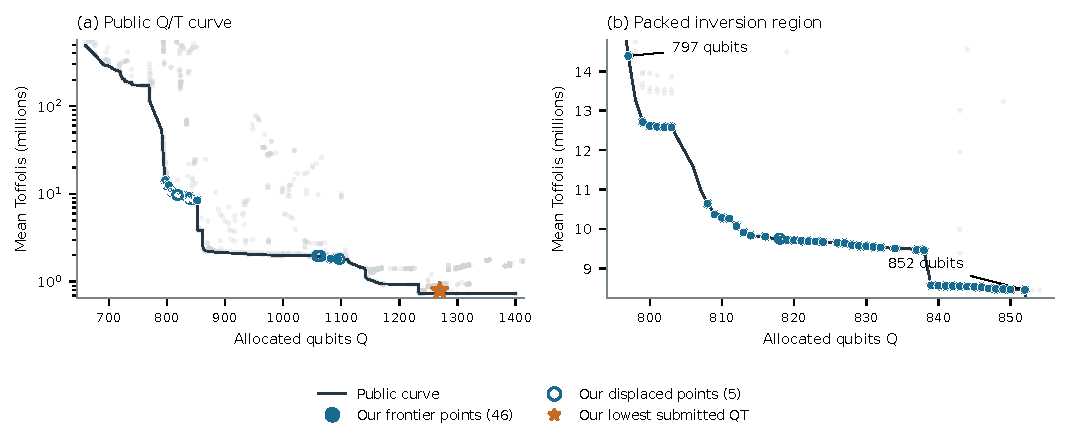
\includegraphics[width=\textwidth]{figures/fig1_overview.pdf}
\caption{\textbf{Our circuits on the ECDSA.fail frontier.}
(a) The public Q/T frontier at 12:05 UTC on 26 October 2026.
Blue points mark our 46 frontier coordinates at the cutoff; open points mark our five displaced coordinates.
The star marks our lowest submitted $QT$, which lies outside the public frontier.
(b) Detail of the packed-inversion region at 797--852 qubits.}
\label{fig:overview}
\end{figure*}

\section{ECDSA.fail leaderboard results}
The qubit--Toffoli Pareto curve compares circuits across workspace budgets: each point offers a tradeoff between the two resources.
Our pipeline contributes 46 of its 215 points, a share of 21.4\% (Figure~\ref{fig:overview}, Table~\ref{tab:contributors}).
These circuits span 797--1095 qubits and 1.818--14.390 million mean Toffolis.
Forty-four points build on collaborators' packed Euclidean inversion circuits, nicknamed \emph{Froghop}, which share storage between shrinking remainders and growing inverse coefficients.
We extend this family through measurement-based cleanup, exact replacements of short gate blocks, and changes to workspace allocation.

\begin{table*}[!tp]
\caption{\textbf{Frontier shares at the 26 October, 12:05 UTC snapshot.}
Each coordinate belongs to its earliest published entry; frontier share divides by 215 coordinates.
Successful commits gives the fraction of distinct submitted commits on this frontier.
Our 52 submissions have distinct commits; 46 remain on the frontier (88.5\%).
Submissions include repeated commits and exclude unpublished trials.}
\label{tab:contributors}
\centering
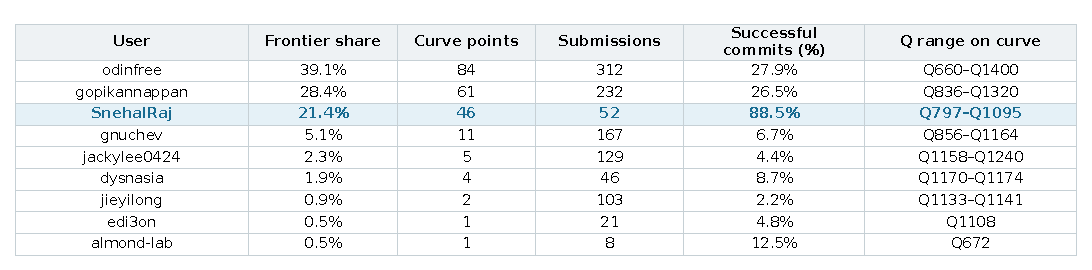
\includegraphics[width=\textwidth]{figures/table_frontier_contributors.pdf}
\end{table*}

\begin{table*}[!tp]
\caption{\textbf{Resource reductions across the three families we modify.}
Rows order the largest Toffoli reductions from high to low.
Each saving compares a submitted circuit with its declared parent; Leapfrog uses our repaired control.
T differences use recorded rounded means on separate evaluation inputs.
The two maxima can describe different circuits.
The largest Froghop T saving adds 20 qubits; its largest Q saving adds 1,811,710 Toffolis.
The largest SKY-COF Q saving adds 85,793 Toffolis.
The Leapfrog circuit saves both 22 qubits and 63,584 Toffolis from the repaired control.
Commits / curve gives measured commits and their points on the frozen frontier.
All 52 submissions have published resource counts.}
\label{tab:ownfamilies}
\centering\small
\begin{tabular}{p{.11\textwidth}p{.30\textwidth}rrrr}
\toprule
Family & Edits & Commits / curve & Q range & Max. T saving & Max. Q saving \\
\midrule
Froghop & Cleanup, gate replacement, and workspace allocation & 45 / 44 & 797--852 & 271,963 & 6 \\
Leapfrog & Approximation tuning after reliability repair & 1 / 0 & 1270 & 63,584 & 22 \\
SKY-COF & Gate replacement and cofactor storage & 6 / 2 & 1059--1097 & 1,119 & 6 \\
\bottomrule
\end{tabular}

\end{table*}

Table~\ref{tab:ownfamilies} groups our measured submissions by arithmetic family and reports their largest resource reductions.
Within packed inversion, extra carry storage saves up to 271,963 published mean Toffolis at a cost of 20 qubits.
Cleanup and exact gate replacements also reduce Toffolis at fixed width; a paired 818-qubit test isolates a 20,206-Toffoli saving from gate replacements.
The other two frontier points use circuits that store inverse coefficients in shared workspace, nicknamed \emph{SKY-COF}.
Gate replacements save Toffolis at fixed width, while changes to cofactor storage save up to six qubits with more arithmetic.
Gate replacements give frontier points at 1,082 and 1,095 qubits.

Our lowest leaderboard submission has $QT=1{,}008{,}123{,}460$, from 1,270 qubits and 793,798 mean Toffolis.
It descends from a family that couples an inversion walk with arithmetic replay, nicknamed \emph{Leapfrog}.
We first make its approximation settings more conservative to reduce failures, then tune precision, traversal length, and workspace to recover resource cost.
The selected circuit reduces $QT$ by 8.99\% from the repaired 1,292-qubit control (Table~\ref{tab:product}).
On 32,768 matched inputs, the public parent, repaired control, and selected circuit fail 92, one, and nine times, respectively.
The selected circuit therefore spends some of the reliability margin gained by the repair to reduce cost.
Against the fixed 24 October public comparator, it has ninefold lower observed failure rate at a 10.10\% higher resource product.
A separate audit on 262,144 fresh inputs gives a failure-rate bound of 0.0406\%, rounded upward.
Section~\ref{sec:approximation} defines the observed failure rate and its statistical bound.



\section{Methods}
\subsection{Point-addition benchmark}
ECDSA.fail tests point addition over the secp256k1 field, with modulus $p=2^{256}-2^{32}-977$~\cite{openauto}.
The circuit adds a point given as classical input to a point held in a quantum register.
The circuit must compute the sum, preserve the specified inputs, clear scratch qubits, and cancel unwanted phase.
Reversible Boolean gates, phase operations, and measurement/reset allow efficient classical simulation of these checks.
For mean executed Toffolis $\overline{T}$, the score is
\begin{equation}
T=\lfloor\overline{T}+0.5\rfloor,\qquad S=QT.
\end{equation}
The mean depends on the evaluation inputs.
The score excludes hardware routing, error correction, and measurement latency.

\begin{table*}[!tp]
\caption{\textbf{Arithmetic families in the public sources.}
The public aliases identify the source lineages used in our analysis.}
\label{tab:families}
\centering\small
\begin{tabular}{p{.21\textwidth}p{.18\textwidth}p{.52\textwidth}}
\toprule
Family & Public alias & Main mechanism \\
\midrule
Quotient recomputation & Frogdrop & Retain fewer quotient bits and regenerate omitted work; trade storage for more arithmetic. \\
Packed Euclidean walk & Froghop & Pack remainder and cofactor state; choose one-hop or two-hop updates and reuse the shared boundary. \\
Cross-packed divsteps & Lilypad & Use divsteps in packed rings; tune run storage and exploit known-zero cofactor bits. \\
Shared cofactor frame & SKY-COF & Carry cofactors in one frame; adjust rail widths and history allocation. \\
Recycled-history walk & Skywalk & Store decisions in wires released during arithmetic. \\
Coupled walk and replay & Leapfrog, Spookyfrog & Couple inversion progress and payload work; adjust fusion, precision, horizon, and workspace. \\
Recorded Euclidean replay & Dialog, Jump-2, PingPong & Store a compact decision transcript and replay it; compress decisions or alternate registers. \\
\bottomrule
\end{tabular}
\end{table*}

\subsection{Public data and source selection}
We collect 2,211 public submissions at the cutoff, including resource counts, research notes, source commits, and evaluation results.
We use these records to identify the main frontier approaches (Table~\ref{tab:families}, Figure~\ref{fig:families}).
We use circuit implementations from the supplemental repository~\cite{supplementrepo}.

We fix the source versions before each experiment and record their settings and authors.
The compiler study keeps inherited approximation settings fixed; the separate product search varies those settings.

\begin{figure*}[!tp]
\centering
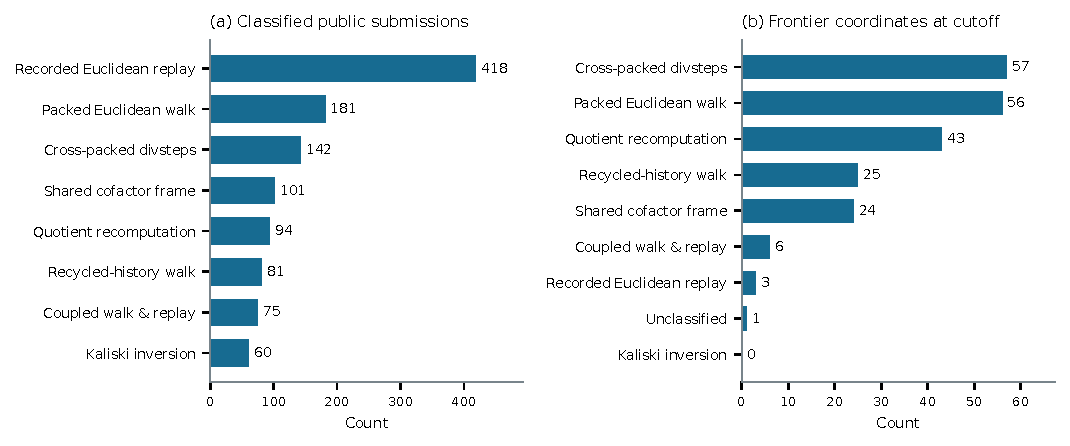
\includegraphics[width=\textwidth]{figures/fig3_families.pdf}
\caption{\textbf{Circuit families named in public notes.}
(a) The 1,152 submissions with identified families among 1,778 validated results, including repeated submissions.
(b) All 215 frontier coordinates, including one with an unidentified family.
Each panel orders families by decreasing count.
Panel (a) omits 626 unclassified submissions.
The labels come from submission notes.}
\label{fig:families}
\end{figure*}

\subsection{Packed inversion and our edits}
Froghop implements modular inversion through a reversible extended Euclidean algorithm~\cite{froghopsources}.
Cofactors record the coefficients needed to recover the modular inverse.
Each of two registers stores a remainder and a cofactor from opposite ends.
Shrinking remainders leave space for growing cofactors, which reduces the storage needed for inversion.
A shared boundary tracks their separation, while quotient bits control the cofactor updates.
The one-hop version combines a cofactor update with alignment for the next division; the two-hop version performs these stages separately.
Our 44 packed-inversion frontier points use both versions: six circuits at 797--803 qubits use two-hop updates; the remaining 38 use one-hop updates.

For a quantum point $(x,y)$ and classical addend $(x_0,y_0)$, the circuit first forms $d=x-x_0$ and $e=y-y_0$.
Froghop inversion computes the slope $\lambda=e/d$.
The coordinate products then give $d'=\lambda^2-d-3x_0$ and $n=-\lambda d'$.
A second inversion recovers $\lambda=-n/d'$ to repair the phase after slope erasure.
The output is $(x',y')=(d'+x_0,n-y_0)$, with all arithmetic modulo $p$ and nonzero division denominators.
Figure~\ref{fig:froghop} shows these circuit blocks and an AND cleanup used by our edits.

Our cleanup edits enable \code{u} and \code{r} where the parent omits them.
Option \code{u} measures an AND value and repairs its phase; option \code{r} absorbs unread writes before measurement/reset into phase operations.
The inherited arithmetic, traversal schedules, approximation settings, and nonces stay fixed.
We apply these passes to the emitted circuits, then run the public checker and fresh audits.
The compiler-pass study below measures the isolated and combined savings.

The gate-replacement and layout edits use the 818- and 839-qubit one-hop constructions and the 803-qubit two-hop construction~\cite{frontierextensions}.
The catalog replaces short blocks on three or four wires with cheaper blocks that have the same signed permutation.
It saves 20,206 Toffolis in the Q818 paired test.
We vary scratch-pool sizes and carry-lane counts to obtain different qubit--Toffoli tradeoffs.
The carry-lane edits preserve ordinary majority-gate lanes during the second inversion, as required by its rolling prefix and inverse repair.
These edits preserve the inherited nonce and approximation settings.

\begin{figure*}[!tp]
\centering
\resizebox{\textwidth}{!}{% Circuit blocks follow the frozen one-hop and two-hop Froghop sources.
% Panel (b) shows the simplest instance of conditional-AND option u.
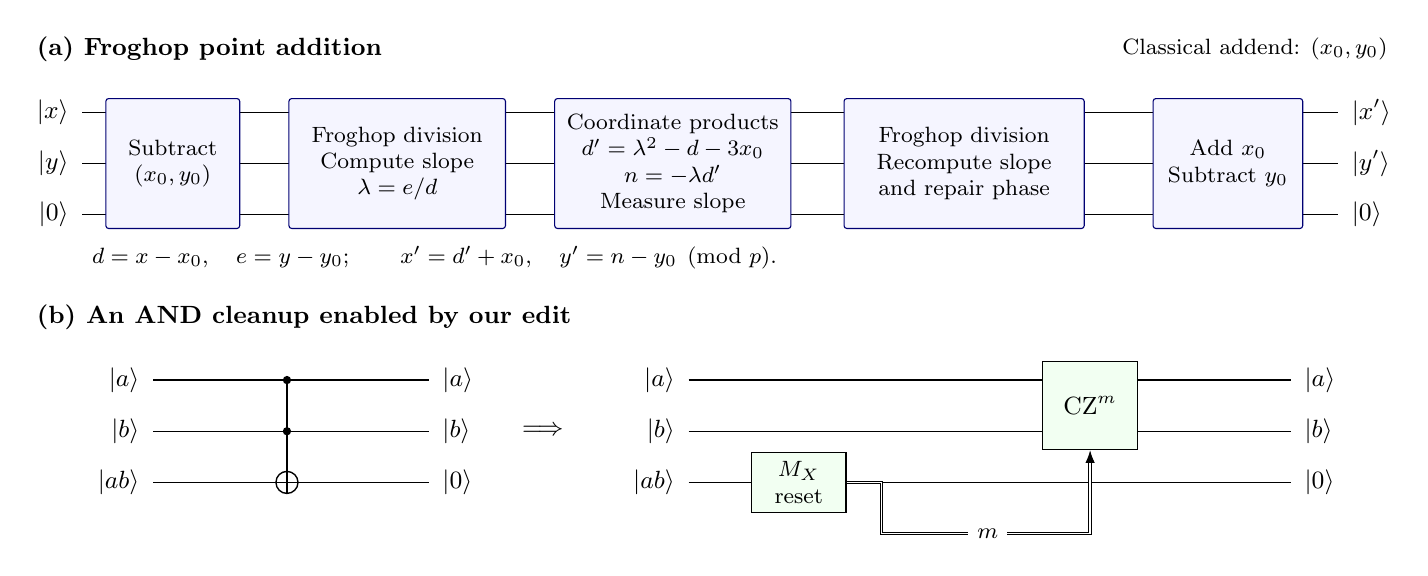
\begin{tikzpicture}[x=1cm,y=1cm,
  every node/.style={font=\small},
  block/.style={draw=blue!45!black,fill=blue!4,rounded corners=1pt,
    align=center,minimum height=1.65cm,inner sep=3pt,font=\footnotesize},
  wire/.style={line width=.5pt},
  classical/.style={double,double distance=.6pt,line width=.35pt,-{Latex[length=1.6mm]}}]
\node[anchor=west,font=\small\bfseries] at (0,4.6) {(a) Froghop point addition};
\node[anchor=east,font=\footnotesize] at (17.4,4.6) {Classical addend: $(x_0,y_0)$};
\foreach \y/\left/\right in {3.8/x/x',3.15/y/y',2.5/0/0} {
  \draw[wire] (.7,\y)--(16.65,\y);
  \node[anchor=east] at (.65,\y) {$|\left\rangle$};
  \node[anchor=west] at (16.7,\y) {$|\right\rangle$};
}
\node[block,minimum width=1.7cm] at (1.85,3.15) {Subtract\\$(x_0,y_0)$};
\node[block,minimum width=2.75cm] at (4.7,3.15) {Froghop division\\Compute slope\\$\lambda=e/d$};
\node[block,minimum width=3.0cm] at (8.2,3.15) {Coordinate products\\$d'=\lambda^2-d-3x_0$\\$n=-\lambda d'$\\Measure slope};
\node[block,minimum width=3.05cm] at (11.9,3.15) {Froghop division\\Recompute slope\\and repair phase};
\node[block,minimum width=1.9cm] at (15.25,3.15) {Add $x_0$\\Subtract $y_0$};
\node[anchor=west,font=\footnotesize] at (.7,1.95)
  {$d=x-x_0,\quad e=y-y_0;\qquad x'=d'+x_0,\quad y'=n-y_0\pmod p$.};

\node[anchor=west,font=\small\bfseries] at (0,1.2) {(b) An AND cleanup enabled by our edit};
\begin{scope}[shift={(.8,-1.1)}]
  \foreach \y/\v in {1.5/a,.85/b} {
    \draw[wire] (.8,\y)--(4.3,\y);
    \node[anchor=east] at (.75,\y) {$|\v\rangle$};
    \node[anchor=west] at (4.35,\y) {$|\v\rangle$};
    \fill (2.5,\y) circle (1.5pt);
  }
  \draw[wire] (.8,.2)--(4.3,.2);
  \node[anchor=east] at (.75,.2) {$|ab\rangle$};
  \node[anchor=west] at (4.35,.2) {$|0\rangle$};
  \draw[wire] (2.5,1.5)--(2.5,.06);
  \draw[wire,fill=white] (2.5,.2) circle (.14);
  \draw[wire] (2.36,.2)--(2.64,.2) (2.5,.06)--(2.5,.34);
  \node at (5.75,.85) {$\Longrightarrow$};

  \foreach \y/\v in {1.5/a,.85/b} {
    \draw[wire] (7.6,\y)--(15.25,\y);
    \node[anchor=east] at (7.55,\y) {$|\v\rangle$};
    \node[anchor=west] at (15.3,\y) {$|\v\rangle$};
  }
  \draw[wire] (7.6,.2)--(15.25,.2);
  \node[anchor=east] at (7.55,.2) {$|ab\rangle$};
  \node[anchor=west] at (15.3,.2) {$|0\rangle$};
  \node[draw,fill=green!5,align=center,minimum width=1.2cm,
    minimum height=.65cm,font=\footnotesize] (measure) at (9,.2) {$M_X$\\reset};
  \node[draw,fill=green!5,minimum width=1.2cm,minimum height=1.12cm] (phase) at (12.7,1.175) {$\mathrm{CZ}^{m}$};
  \draw[classical] (measure.east)--(10.05,.2)--(10.05,-.45)--(12.7,-.45)--(phase.south);
  \node[fill=white,font=\footnotesize] at (11.4,-.45) {$m$};
\end{scope}
\end{tikzpicture}
}
\caption{\textbf{Froghop point addition and the cleanup used in our submissions.}
(a) Circuit blocks follow the frozen source constructors~\cite{froghopsources}; the third wire groups the temporary qubits.
The division blocks include forward and reverse Euclidean traversals.
Measurement and later phase repair allow the circuit to reuse registers.
(b) The simplest instance of option \code{u} replaces a Toffoli erasure of $ab$ with X-basis measurement, reset, and $\mathrm{CZ}^{m}$.
The measurement result $m$ controls the phase repair; both operand values must remain available~\cite{gidney,gidneyblog}.
Our edits change the cleanup passes around the inherited arithmetic.}
\label{fig:froghop}
\end{figure*}

\subsection{Approximation tuning and evaluation inputs}
\label{sec:approximation}
An \emph{approximation setting} limits arithmetic resources while permitting failure on rare inputs.
Examples include a finite walk horizon and a narrowed comparison window.
We tune these settings to balance resource cost against the \emph{observed failure rate}, the fraction of independent inputs that fail any required check.
Each input uses two measurement streams and counts as failed if either stream fails.
We report a \emph{failure-rate bound} to account for uncertainty from the finite sample.
For $k<n$ failures in $n$ inputs, the one-sided exact binomial bound is
\begin{equation}
U=\operatorname{Beta}^{-1}(1-\alpha;k+1,n-k).
\end{equation}
Throughout this work, the joint-check audit limit is $U\le0.001$.
Within each declared group of $m$ planned audits, we allocate $\alpha=0.05/m$ to give that group simultaneous 95\% coverage.
The packed-inversion audit records reserve $m=32$ per group; the matched public panel uses $m=16$, and the larger product confirmation uses $m=2$.
The fine-tuning pilot uses a separate provisional classical-only screen, described in Section~\ref{sec:finetuning}.

The public evaluator derives 9,024 shots from the serialized circuit hash~\cite{openauto}.
A \emph{nonce} changes that hash through redundant operations.
Searching nonces can select a clean public test without changing the circuit's independent failure probability.
Arithmetic edits also change the hash, so we audit selected circuits on fresh inputs (Table~\ref{tab:product}).

The packed-inversion edits preserve each parent's approximation settings and nonce.
The lowest-$QT$ circuit instead uses settings selected by our search.
For arithmetic-variant screening, we run the public evaluator once per distinct variant.
In the screening study frozen on 25 October, 19 of 31 shared-frame and Froghop tests pass and 12 fail.
The parents contain nonce values selected by their authors.
Our audits use independent inputs after candidate selection.

\begin{table}[t]
\caption{\textbf{Resource cost and observed failures.}
The 1,292-qubit control uses more conservative arithmetic settings than the Leapfrog parent.
Resource counts come from the recorded evaluation for each circuit.
Failures use the same 32,768 inputs, with two measurement streams per input.}
\label{tab:product}
\centering\small
\begin{tabular}{lrrrr}
\toprule
Circuit & Q & T & $QT/10^9$ & Failures \\
\midrule
24 Oct. comparator & 1,234 & 742,031 & 0.9157 & 81 \\
Leapfrog parent & 1,236 & 768,542 & 0.9499 & 92 \\
Control & 1,292 & 857,382 & 1.1077 & 1 \\
Our lowest $QT$ & 1,270 & 793,798 & 1.0081 & 9 \\
\bottomrule
\end{tabular}
\end{table}

\begin{figure*}[!tp]
\centering
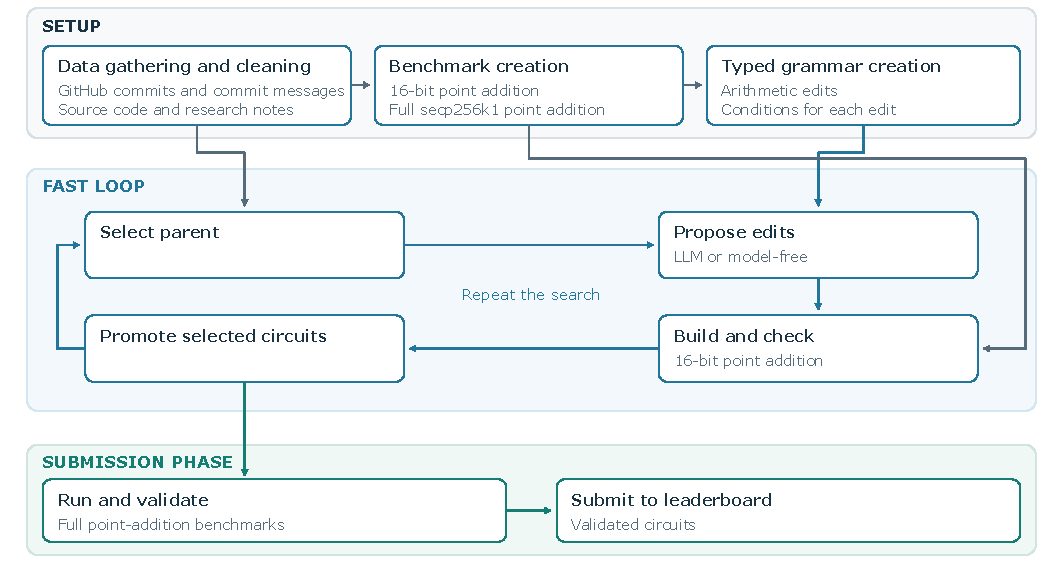
\includegraphics[width=\textwidth]{figures/fig2_pipeline.pdf}
\caption{\textbf{Design of the staged point-addition search.}
The fast loop uses full 16-bit point addition; the submission phase uses optimized secp256k1 constructors.
Model-free search and optional Claude or GPT feedback share the edit interface.
Shared rewrites need an implementation at both stages.
Full-width layout settings use the secp256k1 stage directly and record why they have no small-stage mapping.
Selected circuits undergo reference checks and fresh audits before submission.
Audit inputs remain separate from development inputs.
The experiments evaluate the components separately.
The model comparison uses the full 16-bit environment.}
\label{fig:pipeline}
\end{figure*}

\subsection{Search and submission pipeline}
Figure~\ref{fig:pipeline} connects the setup, fast search loop, and submission phase.
The following steps use the same edit interface with or without model feedback.

\noindent\textbf{Build the benchmarks.}
The fast stage tests full 16-bit point addition with Kaliski inversion; the submission phase tests optimized secp256k1 circuits.
Both evaluators check coordinates, phase, scratch, and preservation of the classical input point (Table~\ref{tab:timing}).



\noindent\textbf{Define legal edits.}
Each grammar rule records its source, applicability conditions, implementation, and known counterexamples.
Shared rewrites need implementations at both widths; layout settings without a 16-bit counterpart run directly at full width.

\noindent\textbf{Select a parent and propose edits.}
Model-free evolution selects a parent that passes the development checks and applies a legal grammar edit.
The model-assisted version also receives edit recommendations based on evaluation feedback; both versions retain valid circuits as possible parents.

\noindent\textbf{Build and check.}
The fast evaluator checks each candidate's coordinates, phase, scratch, and classical input point.
Invalid and duplicate proposals consume their search slots.

\noindent\textbf{Retain and promote.}
Valid circuits remain available as parents, and selected Q/T tradeoffs advance to full-width evaluation.
Each full-width candidate needs its own checks and fresh audit, including edits that have no small-stage implementation.

\noindent\textbf{Audit before submission.}
We freeze each selected circuit before testing fresh inputs under the joint-check protocol in Section~\ref{sec:approximation}.

\noindent\textbf{Submit and record the result.}
We check the live curve before submitting a qualifying candidate from its frozen source checkout.
The submission record links the parent, edits, audits, and leaderboard result.

\begin{table*}[!tp]
\caption{\textbf{Validation of full point addition on 100,000 input pairs per circuit.}
Each pair uses two measurement streams.
Time covers validation and excludes circuit generation and compilation.
The runs use an Apple M2 workstation with eight cores and 24 GiB of memory.
The 16-bit circuit uses Kaliski inversion with policy \code{mfsur}; the secp256k1 circuit is our lowest-$QT$ Leapfrog circuit.
Mean T uses the timing inputs.}
\label{tab:timing}
\centering\small
\pendingtable{timing-table.tex}
\end{table*}

\noindent\textbf{Grammar study.}
We enumerate the 16 combinations of two cleanup options, cofactor-register release, and a combined coordinate construction on one 16-bit Kaliski parent.
Nested grammars separate the cost reduction available from each edit class (Table~\ref{tab:grammar}, Figure~\ref{fig:ablations}a).
Cleanup reduces $QT$ by 11.70\%; adding register release raises that reduction to 18.60\%.

\begin{table*}[!tp]
\caption{\textbf{Cost reachable with each point-addition grammar.}
All rows start from the same parent after the common \code{mfs} compiler preparation.
G0 enables cleanup options \code{u} and \code{r}; G1 adds cofactor-register release; G2 also permits combined coordinate products.
We enumerate every combination and report each grammar's lowest $Q\overline{T}$ among circuits that pass the joint-check audit.
Gain measures the reduction from the prepared parent, excluding common preparation.
Common preparation reduces the original parent's cost by 5.81\%.
All costs use the same fresh audit inputs and mean executed Toffolis before rounding.}
\label{tab:grammar}
\centering\small
\pendingtable{point-addition-grammar-table.tex}
\end{table*}

\begin{figure*}[!tp]
\centering
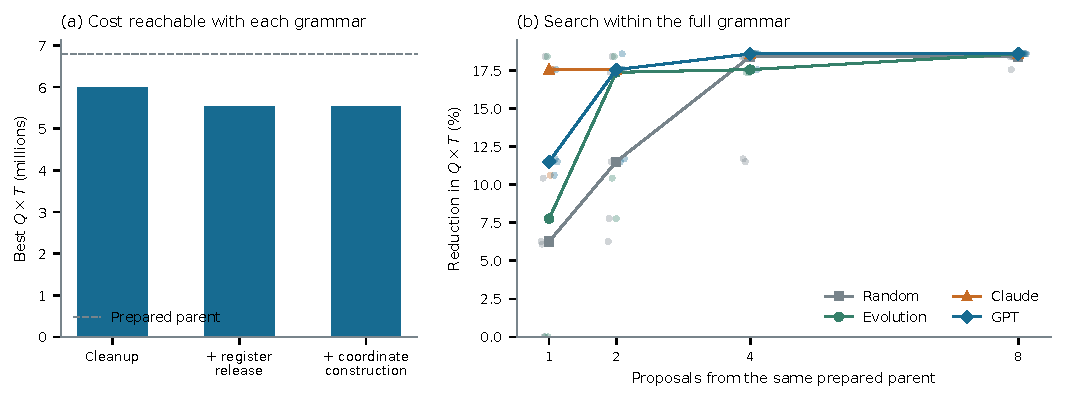
\includegraphics[width=\textwidth]{figures/fig4_ablations.pdf}
\caption{\textbf{Grammar capacity and search efficiency on full 16-bit point addition.}
(a) The lowest resource cost that passes the joint-check audit in each nested grammar.
(b) Best cost reduction after 1, 2, 4, and 8 proposals within the full grammar.
Lines show medians over five runs; faint points show individual runs.
Every run starts from the same prepared parent.
Each method chooses two proposals before receiving their evaluation results.}
\label{fig:ablations}
\end{figure*}

\noindent\textbf{Model comparison.}
Random search, evolution, Claude, and GPT each receive eight proposals from the same grammar, parent, and paired input sets (Table~\ref{tab:model}).
Models see rule descriptions and past evaluations; they receive no results from the exhaustive grammar study.
Claude's first proposal reduces $QT$ by 17.57\% at the median, compared with 7.77\% for evolution.
By eight proposals, evolution and both models share the same 18.60\% median reduction.

\begin{table*}[!tp]
\caption{\textbf{Search from one full 16-bit point-addition parent.}
Values are median reductions in $Q\overline{T}$ across five paired runs, measured from the prepared parent.
Best by 4 or 8 counts runs that find the grammar's minimum within that budget.
Evolution favors one-setting edits; random search samples all unseen recipes uniformly.
Models choose from the same unseen recipes, with feedback after each pair.
Failed calls consume slots; Calls reports completed/attempted counts.
The CLIs retain their default contexts; GPT's resolved model ID is unreported.
The five runs vary input packets and menu order; the subscription CLIs do not expose a sampling seed.
All 17 circuits have zero failures on 16,384 fresh inputs after finalists freeze.
At $\alpha=0.05/20$, each failure-rate bound is 0.0366\%, rounded upward.}
\label{tab:model}
\centering\small
\pendingtable{point-addition-model-table.tex}
\end{table*}

\noindent\textbf{Compiler study.}
We apply gate replacements, Boolean factoring, and algebraic cancellation to 36 public sources (Figure~\ref{fig:passes}).
Paired checks compare parent and child; measured cleanup must also repair phase while the required operands remain available~\cite{gidney,gidneyblog}.

\begin{figure*}[!tp]
\centering
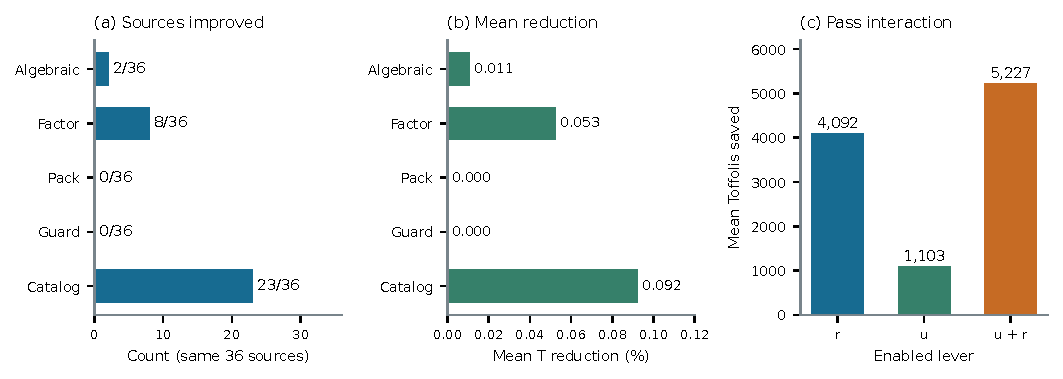
\includegraphics[width=\textwidth]{figures/fig3_strategies.pdf}
\caption{\textbf{Compiler-pass opportunities in public circuits.}
(a) Sources with lower T after each pass.
(b) Mean percentage reduction across all 36 sources, including unchanged circuits.
(c) Isolated and combined cleanup options on the same 839-qubit parent.
All comparisons use the same 8,192-input development protocol.}
\label{fig:passes}
\end{figure*}

\section{Limitations}
We now document what fell short in fine-tuning and what prevented us from extending the search to new arithmetic families.
The fine-tuning study found transferable setting changes but produced few usable edits.
Our executable grammar likewise supports local improvements, while broader arithmetic rules still require implementations and checks.
These outcomes suggest separate next steps for reliable proposal generation and for a larger space of circuit designs.

\subsection{Fine-tuning study}
\label{sec:finetuning}
We fine-tune Qwen2.5-Coder-7B-Instruct on recorded circuit edits to test whether it can propose useful changes on held-out parents~\cite{finetuning}.
The study compares supervised training, feedback during search, and further training on model-generated examples (Table~\ref{tab:finetuning}).
We also train on frontier examples that pair source changes with resource measurements, using a control with the same adapter rank.
These experiments ask whether examples of successful edits teach the model which arithmetic settings affect cost.

Two obstacles limit the resulting proposals.
First, settings in the source can leave the selected constructor unchanged.
A probe finds that only 20 of 206 tested settings change the circuit.
Second, many generated edits either fail to compile or leave the emitted circuit unchanged.
Only 7.8\% of outputs in the self-generated training study both compile and change the circuit.
This leaves too few useful examples for the planned training round.
Adding evaluation feedback also gives zero accepted edits in 48 attempts, compared with one in 48 without feedback.

The setting choices themselves show more promise.
Applying model-discovered changes through a script yields 34 provisionally accepted edits across 13 held-out parents; random setting moves yield zero in 111 attempts.
This suggests separating the choice of an arithmetic setting from the code change that implements it.
A model could select a setting and direction, while a checked transformation applies the edit and records its effect on the circuit.
Figure~\ref{fig:finetuning} places this proposal step within a training and evaluation loop.

The strongest retained control candidate reduces $QT$ by $2.12\times10^6$ and has 108 classical failures in 72,192 inputs, an observed rate of 0.1496\%.
The pilot accepts a classical failure rate up to 0.15\%; phase and scratch failures are outside that provisional screen.
Its accepted edits also shorten an inherited traversal horizon, which can exchange reliability for cost.
We therefore leave independent joint-check audits and paired ablations of the setting changes and traversal length for future work.
The frontier-example arm reaches one parent with provisional improvements, compared with three for the rank-matched control in the incomplete evaluation.
A larger held-out study can test whether the proposed separation improves edit yield and whether frontier examples add useful information.

\begin{table*}[!tp]
\caption{\textbf{Fine-tuning experiments and their outcomes.}
Accepted edits use the provisional classical-only screen described in the text.
The frontier-example comparison is incomplete.
The public frontier results use deterministic compiler and layout edits.}
\label{tab:finetuning}
\centering
\begin{tabular}{p{.30\textwidth}p{.63\textwidth}}
\toprule
Experiment & Observed result \\
\midrule
Supervised adapter training & No generated candidate improves its parent's measured score in the initial evaluations. \\
Feedback during search & 0/48 accepted edits with feedback; 1/48 without feedback. \\
Scripted transfer of setting choices & 34/88 accepted edits on 13 parents; random setting moves give 0/111. \\
Training on model-generated examples & 7.8\% compile and change the circuit, below the 10\% study target. \\
Deterministic repair of failed edits & 2/64 edits compile and change the circuit after repair, below the target of five. \\
Frontier examples and rank-16 control & Provisional improvements on one parent versus three for the control. \\
\bottomrule
\end{tabular}
\end{table*}

\begin{figure*}[!tp]
\centering
\resizebox{\textwidth}{!}{% Proposed design. The retained study tested only parts of this process.
% Keep held-out lineages and validation inputs outside the training loop.
\begingroup
\definecolor{ftblue}{RGB}{38,105,145}
\definecolor{ftgreen}{RGB}{41,119,91}
\begin{tikzpicture}[x=1cm,y=1cm,
  every node/.style={font=\fontsize{8}{9.5}\selectfont},
  ftbox/.style={draw=ftblue!75,fill=white,rounded corners=1.5pt,
    align=center,inner sep=4pt,text width=2.65cm,minimum height=.92cm},
  ftcheck/.style={ftbox,draw=ftgreen!75,text width=3.7cm},
  ftarrow/.style={-{Latex[length=1.6mm]},line width=.65pt,draw=ftblue},
  ftevalarrow/.style={ftarrow,draw=ftgreen}]

\node[anchor=west,font=\fontsize{9}{10.5}\selectfont\bfseries]
  at (0,6.05) {Proposed fine-tuning pipeline};
\draw[draw=ftblue!18,fill=ftblue!4,rounded corners=3pt]
  (0,1.3) rectangle (11.4,5.7);
\draw[draw=ftgreen!18,fill=ftgreen!4,rounded corners=3pt]
  (11.85,1.3) rectangle (17.3,5.7);
\node[anchor=west,text=ftblue,font=\fontsize{8}{9.5}\selectfont\bfseries]
  at (.25,5.43) {TRAINING LOOP};
\node[anchor=west,text=ftgreen,font=\fontsize{8}{9.5}\selectfont\bfseries]
  at (12.1,5.43) {INDEPENDENT EVALUATION};

\node[ftbox] (ftdata) at (1.65,4.25)
  {\textbf{Public edits}\\Split by lineage\\Reserve test data};
\node[ftbox] (fttrain) at (5.2,4.25)
  {\textbf{Train adapter}\\Training split only};
\node[ftbox] (ftpropose) at (9.2,4.25)
  {\textbf{Propose edits}\\Training parents};
\node[ftbox,text width=3.0cm,minimum height=1.22cm] (ftbuild) at (9.2,2.35)
  {\textbf{Build and evaluate}\\16-bit, then full width\\$Q\times T$; coordinates,\\phase, scratch, addend};
\node[ftbox] (ftretain) at (5.2,2.35)
  {\textbf{Keep valid edits}\\Better $Q/T$ tradeoffs};
\draw[ftarrow] (ftdata.east)--(fttrain.west);
\draw[ftarrow] (fttrain.east)--(ftpropose.west);
\draw[ftarrow] (ftpropose.south)--(ftbuild.north);
\draw[ftarrow] (ftbuild.west)--(ftretain.east);
\draw[ftarrow] (ftretain.north)--(fttrain.south);
\node[text=ftblue,font=\fontsize{7.5}{9}\selectfont]
  at (7.2,3.3) {Repeat training};

\node[ftcheck] (ftfreeze) at (14.575,4.25)
  {\textbf{Freeze selected model}};
\node[ftcheck] (fttest) at (14.575,3.05)
  {\textbf{Propose edits}\\Held-out parent lineages};
\node[ftcheck,minimum height=1.0cm] (ftaudit) at (14.575,1.88)
  {\textbf{Full-width validation}\\Fresh inputs; same checks\\Report $Q\times T$ and failure};
\draw[ftevalarrow] (fttrain.north)--(5.2,5.02)--(14.575,5.02)--(ftfreeze.north);
\node[fill=white,inner sep=2pt,text=ftgreen,font=\fontsize{7.5}{9}\selectfont]
  at (9.25,5.02) {After model selection};
\draw[ftevalarrow] (ftfreeze.south)--(fttest.north);
\draw[ftevalarrow] (fttest.south)--(ftaudit.north);
\node[anchor=west,font=\fontsize{7.5}{9}\selectfont]
  at (0,.8) {Keep held-out results outside training.};
\end{tikzpicture}
\endgroup
}
\caption{\textbf{Proposed fine-tuning workflow.}
The training loop reuses valid improvements.
Independent evaluation uses a frozen model, held-out lineages, and fresh inputs.
The retained study tested parts of this design with classical-only acceptance.
Small-stage tests apply where the edit has a 16-bit implementation.}
\label{fig:finetuning}
\end{figure*}

\subsection{Search over arithmetic programs}
Our 46 frontier points come from deterministic compiler and layout edits within two existing inversion families.
These edits expose savings in cleanup and storage, while retaining the parent's arithmetic program.
Larger changes require a search space that can alter how the circuit computes and retains intermediate values.
We explored this direction by recording 23 broader arithmetic rules; turning those descriptions into executable transformations remains unfinished work.

The controlled model study motivates testing a larger edit space.
It compares 16 edit combinations on one 16-bit Kaliski constructor.
Model guidance finds good combinations earlier, but evolution reaches the same median gain within eight proposals.
Future comparisons should vary constructors and search budgets, with controls that match the number of edits allowed per proposal.
They can then measure whether the early search gains persist as the grammar grows and at full field width.

We propose a grammar of \emph{typed arithmetic programs} with explicit register roles and block requirements.
Register roles would distinguish field values, carries, cofactors, and retained arithmetic decisions.
The search could then choose between storing an intermediate value, recomputing it, or erasing it through measurement and phase correction.
Measured cleanup makes one dependency especially important: the values needed for later phase correction must remain available.
Tracking this dependency would let the search change storage schedules while preserving the conditions of each cleanup rule.

A first implementation could vary carry storage and cleanup before composing alternative inversion blocks with explicit cofactor tracking.
Each transformation would need an equivalence argument and paired tests of coordinates, phase, scratch, and addend preservation.
Full 16-bit point addition provides a tractable test environment before full-width evaluation.
We leave the discovery of new inversion families to this broader search.

\section{Conclusion}
Our pipeline contributes 46 of 215 public frontier points through cleanup, exact gate replacements, and workspace changes in packed-inversion and shared-cofactor circuits.
Approximation tuning produces a separate circuit with $QT\simeq1.008\times10^9$ and ninefold lower observed failure rate than its fixed 24 October comparator.
The controlled search study shows an early benefit from model guidance within a small edit space, while fine-tuning exposes difficulties in generating usable code changes.
Together, these results motivate checked arithmetic transformations that let models propose changes and let evaluators measure their cost and reliability.
The library packages the edits, search methods, and audit records needed to study that approach.

\section*{AI disclosure}
The author used GPT-6 to help write this manuscript.
The author used Claude Opus and GPT-6 to help develop the research harness.

\section*{Code and data}
The \href{https://github.com/SnehalRaj/quantum-circuit-optimiser}{quantum-circuit-optimiser repository} packages the methods used for the submissions, together with the evaluation harness and experiment records.
The model comparisons use full 16-bit point addition.
The bundle contains source identities, frozen public records, study contracts, outcomes, and vector figures for an offline paper build.
Public constructors retain their authors' licenses and notices.
The lowest-$QT$ circuit descends from \mbox{krishparadox's} Leapfrog submission \code{54acebaf}.
The fixed 24 October comparator is Champollion9012's circuit at commit \code{6b0327d6}.
The Froghop parents come from gnuchev and odinfree; jackylee0424 wrote the conditional-AND passes.
The 1,097-qubit SKY-COF derivative builds on gopikannappan's \code{f22e87ab} and its credited lineage.
The 1,082- and 1,095-qubit derivatives use odinfree's \code{d0abb28f} and \code{8a57279a}, respectively.
The carry-lane derivatives follow gopikannappan's \code{e2194147} setting and guard.

\begin{thebibliography}{9}
\bibitem{openauto}
J.~Long \emph{et al.}, \emph{ECDSA.Fail: Open Autoresearch for Optimizing Elliptic-Curve Point Addition in Shor's Algorithm},
\href{https://arxiv.org/abs/2609.09582v2}{arXiv:2609.09582v2} (2026).
\bibitem{google}
R.~Babbush \emph{et al.}, \emph{Securing Elliptic Curve Cryptocurrencies against Quantum Vulnerabilities: Resource Estimates and Mitigations},
\href{https://arxiv.org/abs/2603.28846v2}{arXiv:2603.28846v2} (2026).
\bibitem{gidney}
C.~Gidney, \emph{Halving the cost of quantum addition}, Quantum \textbf{2}, 74 (2018),
\href{https://doi.org/10.22331/q-2018-06-18-74}{doi:10.22331/q-2018-06-18-74}.
\bibitem{gidneyblog}
C.~Gidney, \emph{Verifying Measurement Based Uncomputation}, Algorithmic Assertions (7 August 2019),
\href{https://algassert.com/post/1903}{algassert.com/post/1903}.
\bibitem{verifiable}
T.~Khattar, N.~C.~Rubin, C.~Gidney, M.~Broughton, G.~H.~Low, and R.~Babbush,
\emph{Leveraging verifiable structure in quantum circuits to find more efficient compilations with agentic AI},
\href{https://arxiv.org/abs/2610.23832v2}{arXiv:2610.23832v2} (2026).
\bibitem{supplementrepo}
J.~Long and contributors, \emph{ECDSA.fail supplemental materials},
\href{https://github.com/jieyilong/ecdsafail-supplemental-materials}{source repository} (accessed 25 October 2026).
\bibitem{froghopsources}
gnuchev and odinfree, \emph{Froghop source constructors and submission notes},
ECDSA.fail (2026), commits \code{410bec6d} and \code{92186c37}.
\href{https://ecdsa.fail/api/submissions/a45bcccd-fb2f-42df-afb9-3412eef8c5df/attribution}{Q839 attribution};
\href{https://ecdsa.fail/api/submissions/b3a70fb3-44c0-4738-9da3-0000cf031c6a/attribution}{Q799 attribution}.
The bundle contains the frozen source files and claim map.
\bibitem{frontierextensions}
SnehalRaj and credited contributors, \emph{Froghop catalog and layout submissions}, ECDSA.fail (2026).
\href{https://ecdsa.fail/api/submissions/b9a40957-b59c-4d8a-90eb-d65831365ec5}{Q818 catalog};
\href{https://ecdsa.fail/api/submissions/1ea65d0c-383f-4060-a141-4f37b5fc34b0}{Q828 carry-lane derivative}.
The frozen snapshot retains the submission notes and their source credits.
\bibitem{finetuning}
S.~Raj, \emph{Circuit candidate-generator fine-tuning study},
commit \code{0f762c895} (2026).
\href{https://github.com/SnehalRaj/quantum-circuit-optimiser/blob/main/studies/historical/finetuning/records/reports/REPORT_v7_v14.md}{Retained experiment report}.
The bundle retains the records and recount.
\end{thebibliography}
\end{document}
